% Generated 2021-02-25 22:49:50 +0530
\subsection{CuttingTool} \label{sec:CuttingTool}


This section provides the semantic information for the \block{CuttingTool} model.

\begin{figure}[ht]
  \centering
    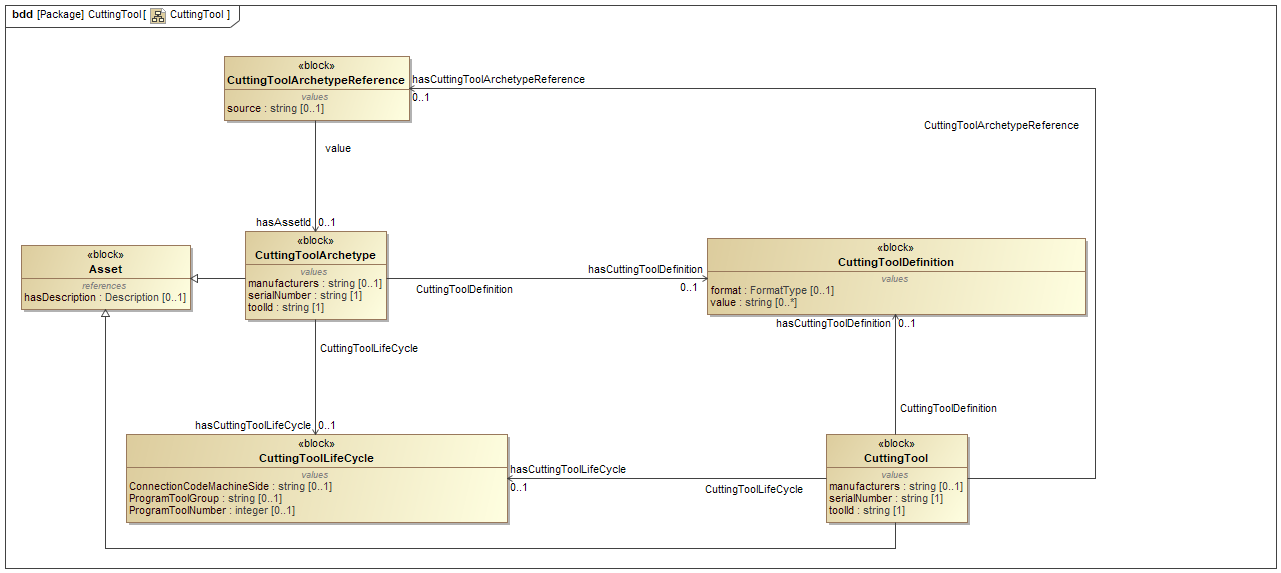
\includegraphics[width=1.0\textwidth]{figures/CuttingTool.png}
  \caption{CuttingTool Diagram}
  \label{fig:CuttingTool Diagram}
\end{figure}

\FloatBarrier


Note: See \sect{CuttingTool Schema Diagrams} for XML schema.



\subsubsection{CuttingTool}




A \block{CuttingTool} physically removes the material from the workpiece by shear deformation.


\paragraph{Attributes of CuttingTool}\mbox{}
\label{sec:Attributes of CuttingTool}

\tbl{Attributes of CuttingTool} lists the attributes of \texttt{CuttingTool}.

\begin{table}[ht]
\centering 
  \caption{Attributes of CuttingTool}
  \label{table:Attributes of CuttingTool}
\tabulinesep=3pt
\begin{tabu} to 6in {|l|l|l|} \everyrow{\hline}
\hline
\rowfont\bfseries {Attribute} & {Type} & {Multiplicity} \\
\tabucline[1.5pt]{}

\property{manufacturers}[CuttingTool] & \texttt{string} & 0..1 \\
\property{serialNumber}[CuttingTool] & \texttt{string} & 1 \\
\property{toolId}[CuttingTool] & \texttt{string} & 1 \\
\end{tabu}
\end{table}
\FloatBarrier

Descriptions for attributes of \block{CuttingTool}:

\begin{itemize}

\item \property{manufacturers}[CuttingTool] \newline The manufacturers of the Cutting Tool.

The representation will be a comma(,) delimited list of manufacturer names.

\item \property{serialNumber}[CuttingTool] \newline The unique identifier for this assembly.

\item \property{toolId}[CuttingTool] \newline The identifier for a class of cutting tools.
\end{itemize}


\paragraph{Elements of CuttingTool}\mbox{}
\label{sec:Elements of CuttingTool}

\tbl{Elements of CuttingTool} lists the elements of \texttt{CuttingTool}.

\begin{table}[ht]
\centering 
  \caption{Elements of CuttingTool}
  \label{table:Elements of CuttingTool}
\tabulinesep=3pt
\begin{tabu} to 6in {|l|l|} \everyrow{\hline}
\hline
\rowfont\bfseries {Element} & {Multiplicity} \\
\tabucline[1.5pt]{}
\texttt{CuttingToolLifeCycle} & 0..1 \\
\texttt{CuttingToolArchetypeReference} & 0..1 \\
\texttt{CuttingToolDefinition} & 0..1 \\
\end{tabu}
\end{table}
\FloatBarrier


Descriptions for elements of \block{CuttingTool}:

\begin{itemize}

\item \block{CuttingToolLifeCycle} \newline Data regarding the application or use of the tool.

This data is provided by various pieces of equipment (i.e. machine tool, presetter) and statistical process control applications. Life cycle data will not remain static, but will change 395 periodically when a tool is used or measured.

\item \block{CuttingToolArchetypeReference} \newline \block{CuttingToolArchetypeReference} has reference information about the \property{assetId} and/or the URL of the data source of \block{CuttingToolArchetype}.

\item \block{CuttingToolDefinition} \newline The \block{CuttingToolDefinition} contains the detailed structure of the Cutting Tool which is be static during its lifecycle. \textit{Ref:ISO 13399}.
\end{itemize}



\subsubsection{CuttingToolArchetype}
\label{sec:CuttingToolArchetype}



The \block{CuttingToolArchetype} represents the static cutting tool geometries and nominal values as one would expect from a tool catalog.


\paragraph{Attributes of CuttingToolArchetype}\mbox{}
\label{sec:Attributes of CuttingToolArchetype}

\tbl{Attributes of CuttingToolArchetype} lists the attributes of \texttt{CuttingToolArchetype}.

\begin{table}[ht]
\centering 
  \caption{Attributes of CuttingToolArchetype}
  \label{table:Attributes of CuttingToolArchetype}
\tabulinesep=3pt
\begin{tabu} to 6in {|l|l|l|} \everyrow{\hline}
\hline
\rowfont\bfseries {Attribute} & {Type} & {Multiplicity} \\
\tabucline[1.5pt]{}

\property{manufacturers}[CuttingToolArchetype] & \texttt{string} & 0..1 \\
\property{serialNumber}[CuttingToolArchetype] & \texttt{string} & 1 \\
\property{toolId}[CuttingToolArchetype] & \texttt{string} & 1 \\
\end{tabu}
\end{table}
\FloatBarrier

Descriptions for attributes of \block{CuttingToolArchetype}:

\begin{itemize}

\item \property{manufacturers}[CuttingToolArchetype] \newline The manufacturers of the Cutting Tool.

The representation will be a comma(,) delimited list of manufacturer names.

\item \property{serialNumber}[CuttingToolArchetype] \newline The unique identifier for this assembly.

\item \property{toolId}[CuttingToolArchetype] \newline The identifier for a class of cutting tools.
\end{itemize}


\paragraph{Elements of CuttingToolArchetype}\mbox{}
\label{sec:Elements of CuttingToolArchetype}

\tbl{Elements of CuttingToolArchetype} lists the elements of \texttt{CuttingToolArchetype}.

\begin{table}[ht]
\centering 
  \caption{Elements of CuttingToolArchetype}
  \label{table:Elements of CuttingToolArchetype}
\tabulinesep=3pt
\begin{tabu} to 6in {|l|l|} \everyrow{\hline}
\hline
\rowfont\bfseries {Element} & {Multiplicity} \\
\tabucline[1.5pt]{}
\texttt{CuttingToolDefinition} & 0..1 \\
\texttt{CuttingToolLifeCycle} & 0..1 \\
\end{tabu}
\end{table}
\FloatBarrier


Descriptions for elements of \block{CuttingToolArchetype}:

\begin{itemize}

\item \block{CuttingToolDefinition} \newline The \block{CuttingToolDefinition} contains the detailed structure of the Cutting Tool which is be static during its lifecycle. \textit{Ref:ISO 13399}.

\item \block{CuttingToolLifeCycle} \newline Data regarding the application or use of the tool.

This data is provided by various pieces of equipment (i.e. machine tool, presetter) and statistical process control applications. Life cycle data will not remain static, but will change 395 periodically when a tool is used or measured.
\end{itemize}



\subsubsection{CuttingToolArchetypeReference}
\label{sec:CuttingToolArchetypeReference}



\block{CuttingToolArchetypeReference} has reference information about the \property{assetId} and/or the URL of the data source of \block{CuttingToolArchetype}.


The value of \texttt{CuttingToolArchetypeReference} \MUST be \texttt{CuttingToolArchetype}.


\paragraph{Attributes of CuttingToolArchetypeReference}\mbox{}
\label{sec:Attributes of CuttingToolArchetypeReference}

\tbl{Attributes of CuttingToolArchetypeReference} lists the attributes of \texttt{CuttingToolArchetypeReference}.

\begin{table}[ht]
\centering 
  \caption{Attributes of CuttingToolArchetypeReference}
  \label{table:Attributes of CuttingToolArchetypeReference}
\tabulinesep=3pt
\begin{tabu} to 6in {|l|l|l|} \everyrow{\hline}
\hline
\rowfont\bfseries {Attribute} & {Type} & {Multiplicity} \\
\tabucline[1.5pt]{}

\property{source}[CuttingToolArchetypeReference] & \texttt{string} & 0..1 \\
\end{tabu}
\end{table}
\FloatBarrier

Descriptions for attributes of \block{CuttingToolArchetypeReference}:

\begin{itemize}

\item \property{source}[CuttingToolArchetypeReference] \newline The URL of the CuttingToolArchetype Information Model.

\end{itemize}



\subsubsection{CuttingToolDefinition}
\label{sec:CuttingToolDefinition}



The \block{CuttingToolDefinition} contains the detailed structure of the Cutting Tool which is be static during its lifecycle. \textit{Ref:ISO 13399}.


The value of \texttt{CuttingToolDefinition} \MUST be \texttt{string}.


\paragraph{Attributes of CuttingToolDefinition}\mbox{}
\label{sec:Attributes of CuttingToolDefinition}

\tbl{Attributes of CuttingToolDefinition} lists the attributes of \texttt{CuttingToolDefinition}.

\begin{table}[ht]
\centering 
  \caption{Attributes of CuttingToolDefinition}
  \label{table:Attributes of CuttingToolDefinition}
\tabulinesep=3pt
\begin{tabu} to 6in {|l|l|l|} \everyrow{\hline}
\hline
\rowfont\bfseries {Attribute} & {Type} & {Multiplicity} \\
\tabucline[1.5pt]{}

\property{format}[CuttingToolDefinition] & \texttt{FormatType} & 0..1 \\
\end{tabu}
\end{table}
\FloatBarrier

Descriptions for attributes of \block{CuttingToolDefinition}:

\begin{itemize}

\item \property{format}[CuttingToolDefinition] \newline Identifies the expected representation of the enclosed data.

\texttt{FormatType} Enumeration:

\begin{itemize}
\item \texttt{EXPRESS} \newline The document will confirm to the ISO 10303 Part 21 standard.
 
\item \texttt{TEXT} \newline The document will be a text representation of the tool data.
 
\item \texttt{UNDEFINED} \newline The document will be provided in an undefined format. 
\item \texttt{XML} \newline The default value for the definition. The content will be an XML document. 
\end{itemize}

\end{itemize}


